%%
% Questions:
% * Is there only 1 blockchain for everyone or can a company/user have its own blockchain?
% *   there are some public blockchains, does it mean there are private ones too?
% => private and public
% * The size grows exponentially, what happens when it's too big?
% => ?
% * Double spending problem example -- solution.
% => timestamps
% * Why is trusted third party not needed?
% => decentralized, hard to alter
%%

\begin{frame}{Blockchain}
  \begin{block}{History}
    \begin{itemize}
      \item 1991: Stuart Haber and W. Scott Stornetta, documents with timestamps. % no changes
      \item 1992: Bayer, Haber and Stornetta, performance optimization.
      \item 2008: Satoshi Nakamoto, no signing by a trusted party.
      \item 2009: Bitcoin.
      \item 2014: 20GB Bitcoin blockchain.
      \item 2017: 100GB Bitcoin blockchain.
    \end{itemize}
  \end{block}
\end{frame}

\begin{frame}{Blockchain}
  \begin{block}{Characteristics}
    \begin{itemize}
      \item Database, system of records (ledger for cryptocurrency).
      \item Distributed.
      \item Decentralized.
      \item Append-only.
      \item Peer-to-peer network.
      \item Chain of blocks of transactions.
      \item Private key cryptography. % user can have many pairs with many public keys
      \item Public (Bitcoin, Ethereum). 
      \item Private, access is restricted.
    \end{itemize}
  \end{block}
\end{frame}

\begin{frame}{Blockchain}
  \begin{block}{Chain structure}
    \begin{center}
      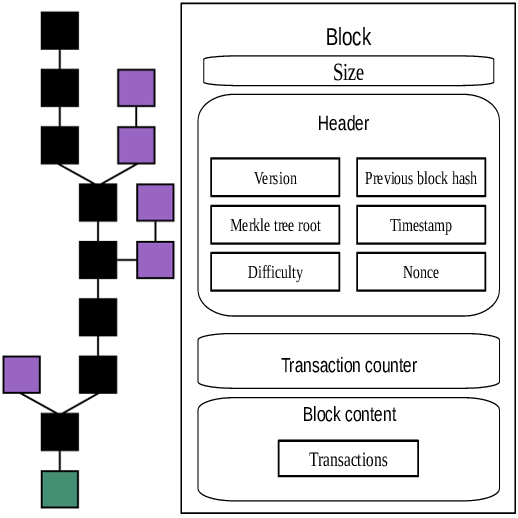
\includegraphics[height=5cm]{img/blockchain.png}
    \end{center}
  \end{block}
\end{frame}

\begin{frame}{Blockchain}
  \begin{block}{Chain}
    \begin{center}
      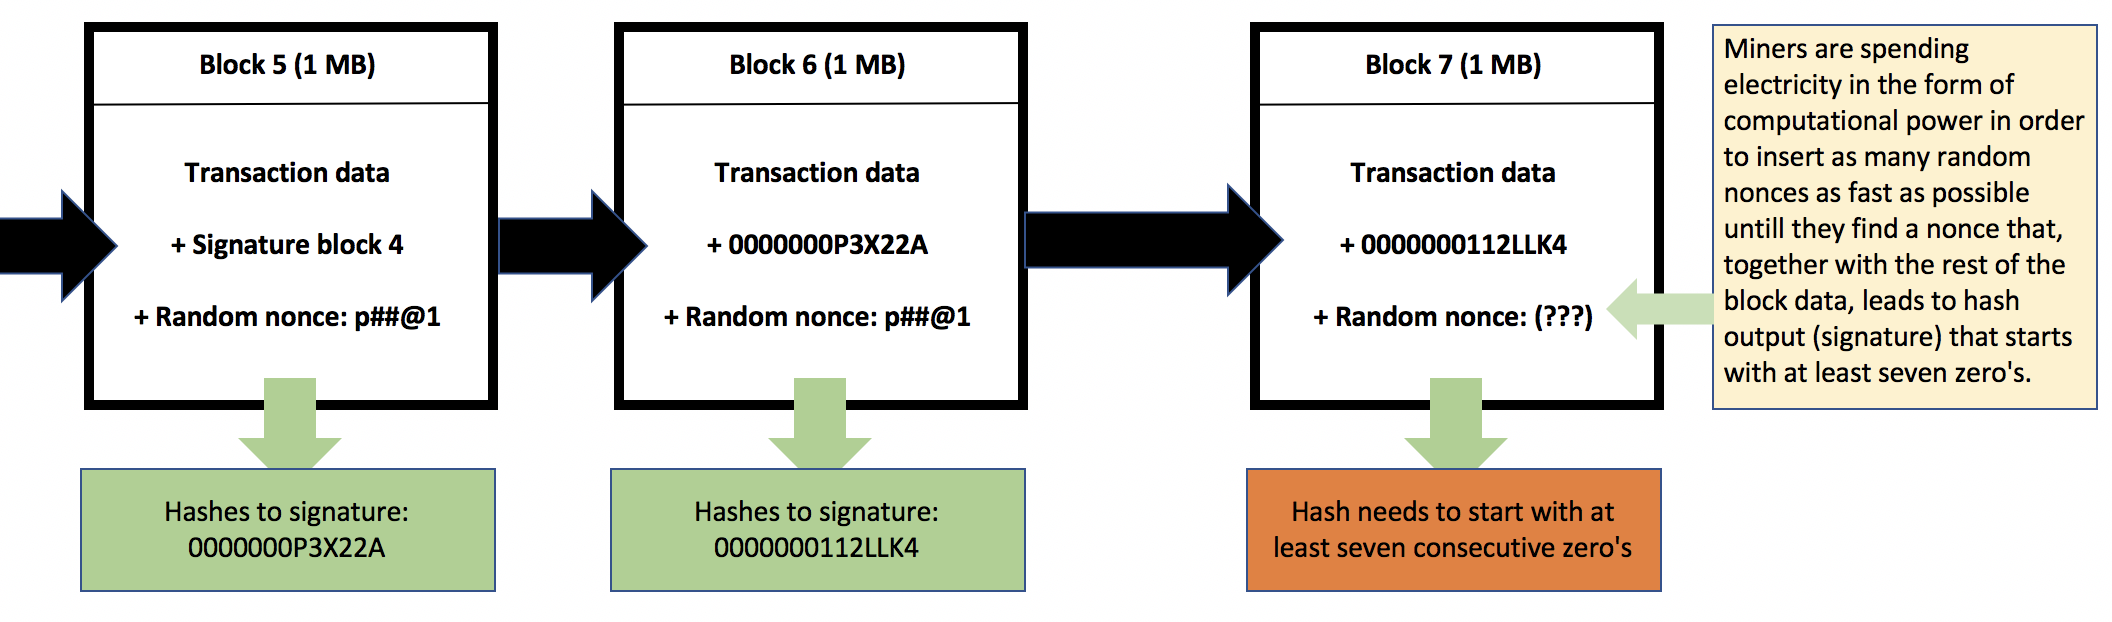
\includegraphics[height=3cm]{img/blocks.png}
    \end{center}
  \end{block}
\end{frame}

\begin{frame}{Blockchain}
  \begin{block}{Principle}
    \begin{itemize}
      \item Transactions (data made by users).
      \item Blocks (confirming records made by miners).
      \item Valid transactions are added to the blockchain.
      \item Validity (user's electronic signature, existing user's wallet with enough money, \dots).
      \item Block time (average time between 2 confirmed blocks).
      \item Shorter block time allows trustworthy transactions (Bitcoin 10m, Ethereum 20s).
    \end{itemize}
  \end{block}
\end{frame}

\begin{frame}{Blockchain}
  \begin{block}{Transaction}
    \begin{center}
      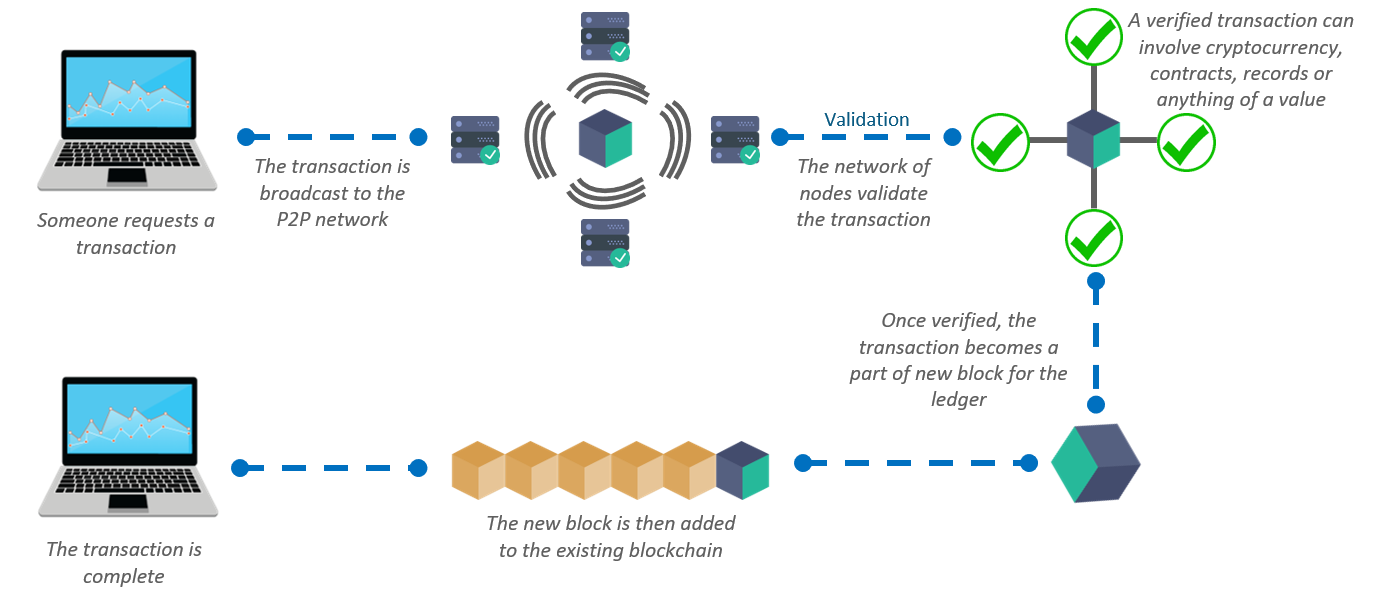
\includegraphics[height=4cm]{img/transaction.png}
    \end{center}
  \end{block}
\end{frame}

\begin{frame}{Blockchain}
  \begin{block}{Advantages}
    \begin{itemize}
      \item Each node has the same power.
      \item Too hard for attackers to edit transactions. % next block requires previous block's hash
      \item Automated conflict solving (invalid transactions will not become part of a blockchain). 
      \item Trusted third party is not needed.
    \end{itemize}
  \end{block}
  \begin{block}{Disdvantages}
    \begin{itemize}
      \item Mining power requirements.
      \item Lacks application development support. 
      \item People do not understand it. 
      \item It can potentially, in theory, replace banks. 
    \end{itemize}
  \end{block}
\end{frame}

\begin{frame}{Blockchain}
  \begin{block}{Examples}
    \begin{itemize}
      \item Cryptocurrency.
      \item Personal documents sharing:ID, visa.
      \item Money transactions among countries.
      \item Medical history/record.
      \item Shipping.
      \item Supply chain monitoring. 
      \item Elections / online voting.
    \end{itemize}
  \end{block}
\end{frame}

\begin{frame}{Blockchain}
  \begin{block}{Decentralization}
    \begin{itemize}
      \item Each node in the network has complete or partial copy.
      \item Each node can check validity of all transactions.
      \item Each node can decide if a transaction is part of a blockchain.
    \end{itemize}
  \end{block}
  \begin{block}{Double spending problem}
    \begin{itemize}
      \item In centralized databases this problem is prevented by operation atomicity.
      \item 2+ nodes create transactions spending (in sum) more than is available.
      \item Solution is based on timestamps and voting for order of transactions (Proof of Work, Proof of Stake).
    \end{itemize}
  \end{block}
\end{frame}

\begin{frame}{Blockchain}
  \begin{block}{Consensus -- Proof of Work}
    \begin{itemize}
      \item Agreement. 
      \item Difficult to generate (mining, energy requirements), easy to validate.
      \item When a node finds a Proof of Work, it completes a block and broatcasts it.
      \item Longest chain wins.
      \item Blocks contain hashes of their parent blocks.
      \item Alternatives: Proof of Stake, Byzantine fault tolerance. 
      \item Protocols: challenge-response, solution-verification.
    \end{itemize}
  \end{block}
\end{frame}

\begin{frame}{Blockchain}
  \begin{block}{Proof of Work -- Challenge-response}
    \begin{center}
      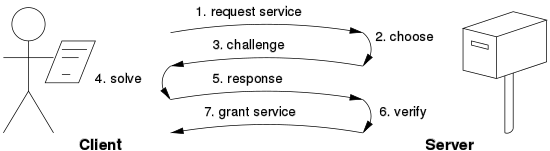
\includegraphics[height=2cm]{img/challenge-response.png}
    \end{center}
  \end{block}
\end{frame}

\begin{frame}{Blockchain}
  \begin{block}{Proof of Work -- Solution-verification}
    \begin{center}
      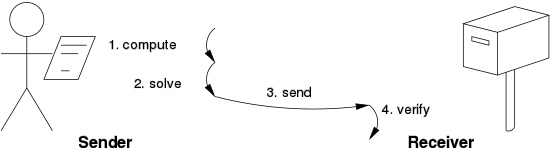
\includegraphics[height=2cm]{img/solution-verification.png}
    \end{center}
  \end{block}
\end{frame}

